%% Begin copyright
%%
%%  /home/jrf/Documents/books/Books20/Docs/Hjs/library.tex
%%
%%   Part of the Books20 Project
%%
%%   Copyright 2022 James R. Fowler
%%
%%   All rights reserved. No part of this publication may be
%%   reproduced, stored in a retrival system, or transmitted
%%   in any form or by any means, electronic, mechanical,
%%   photocopying, recording, or otherwise, without prior written
%%   permission of the author.
%%
%%
%% End copyright


The Harlan J.~Smith Collection of Books at the McDonald Observatory
consists of 511 catalogued entries. However, a number of the entries
refer to multi-volume works or contain multiple reprints and articles
so there are quite a few more than that number of items in the
physical collection.

These works represent only a small part of Harlan's reading
interests.  The collection consists of his science library;
the working books he might have used on a daily basis or for
reference.  Harlan's interests, as indicated by these books, are
primarily in planetary studies and space exploration/development. But
there are also works on math, physics, the history of astronomy,
philosophy of science, life on earth, alien intelligence, and the
colonization of space. There is also a strong interest in climate
change dating back to the 1970's.  The collection includes reports
from his work with the various boards and committees on which he
served, while others are gifts from their authors or interesting
works he picked up in his travels.

\begin{wrapfigure}{r}{0.45\textwidth}
  \centering
  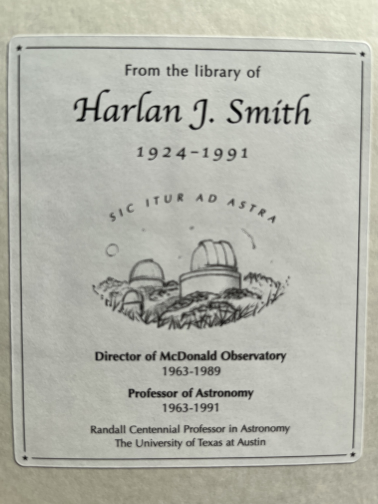
\includegraphics[height=0.34\textheight]{hjs_bookplate_small.png}\\
  {\small Bookplate from the HJS library.\\Designed by Joan Smith.}
  \label{fig:bookplate}
\end{wrapfigure}

Many of the items contain the bookplate {\bfseries\textsc{`From the
    library of} \textit{Harlan J.~Smith'}}, usually on the inside
front cover. This bookplate was designed by Joan Smith and added to
the books when they were first sent to the McDonald Library. The
bookplate shows Mt.~Locke as viewed from the north-east with the
107-inch Harlan J.~Smith telescope in the foreground, the 82-inch Otto
Struve telescope behind it, and the 36-inch telescope in the small
dome to the left.The Latin inscription \textsc{``Sic itur ad astra''}
translates as \textsc{``So we go to the stars''}\footnote{At least
according to \href{https://translate.google.com}{Google Translate}}.

Many of the books also contain the embossed library stamp of Harlan
J.~Smith, usually in the lower-right corner of the title page. These
personalized stamps were quite popular in the 1980s and this stamp was
added by Harlan.

In addition, there is usually a signature or the initials
HJS in the upper-right corner of the front free end paper, though
occasionally they may appear elsewhere.  These ownership marks are
indicated in the catalogue.  Signatures and initials are given as
written in the item.

A number of books appear to have been purchased from used book
dealers.  There are also a number of duplicate books to be found among
all the entries.

The first books were sent to the McDonald library in
1993--94. According to Phil Kelton, Superintendent at the time, the
books were located in his office.  Jane Wiant, who started as the
librarian in 1978, recalls that the collection was later housed in the
HJS telescope building.  At some point the collection was moved to the
Otto Struve library.  When the books arrived in west Texas an
inventory of the collection was created listing 315 items. I have a
paper copy of the Microsoft Excel spreadsheet of this inventory.
Comparison with the 307 items identified in the Struve library for
this catalogue located 300 items on the 1994 inventory. There are also
14 items found in the current catalogue which are not in the 1994
list. Some of these additional items contain the HJS bookplate so they
belong with the collection; other works are relevant to the
observatory so they certainly might belong in this collection. The
counts don't match because some items in the current list are grouped
as one item while they are listed as separate items in the 1994 list.
The inventory work for this catalogue on this group of books was begun
on 1 Dec 2021 and finally finished on 23 Oct 2022, after a long delay.

A second set of books were sent by Nat Smith on 2 November 2021.
Cataloguing occurred 10--11 April 2022. There were 4 boxes and 57
items in this second shipment. A third set of books was received from
Jeffrey Mallon on 29 March 2022. These were catalogued on 9--10 April
2022. There were three boxes and 94 items in the third
shipment. Finally, a fourth shipment was received on 13 April 2022 and
catalogued on 16--17 April 2022. There were two boxes (1 cu ft each)
and one small box (1/2 cu ft) with a total of 54 items in the fourth
shipment.  Work on the software to produce the catalog was started on
18 April 2022 and mostly finished at the end of June 2022. Further
work on the design and layout was incorporated during the proofreading
of the catalogue in the fall of 2022.
\newpage
\noindent
The catalogue entry format is,
\newline

\vbox{%
  \vspace*{0.1 cm}
  \noindent
  {\footnotesize{index}} \textit{Author/Editors(s)} \textsc{\bfseries Title}

year, place, publisher,\hspace{1em}pagination

edition/printing, if known

series name, if a part of a published series

publishing comments

comments about the condition of the item

ownership marks of HJS, if any

HJS catalogue number
}
\hbox{}
\vspace{\parskip} The catalogue is sorted by year and then
author/editor. If there is no note about the binding, then you may
assume a hard-bound book. If there is an intact dust jacket, it is
noted. A paperback book is notated as having paper covers. (Entry
\myhref{98} is interesting; it has paper covers but also a paper dust
jacket as well as a one inch paper ribbon.) Any interesting features
of the item are noted as are any articles by HJS. The HJS catalogue
number is ``HJS Shipment\#.Box\#(0).count'' where shipment 1 is the
existing collection at McDonald while shipments 2, 3, and 4 were the
later boxes shipped in 2021/22. The HJS catalogue number is my
ordering of the books as I catalogued them and form a basic shelf list
that allows me to locate the books again. The 1994 inventory is also
provided in the same format with links to the current
catalogue. Finally, an index of author/editor(s) and the associated
entry number(s) is provided.

